% Options for packages loaded elsewhere
\PassOptionsToPackage{unicode}{hyperref}
\PassOptionsToPackage{hyphens}{url}
\PassOptionsToPackage{dvipsnames,svgnames,x11names}{xcolor}
\documentclass[
  letterpaper,
  11pt]{article}
\usepackage{xcolor}
\usepackage[margin=1in]{geometry}
\usepackage{amsmath,amssymb}
\setcounter{secnumdepth}{-\maxdimen} % remove section numbering
\usepackage{iftex}
\ifPDFTeX
  \usepackage[T1]{fontenc}
  \usepackage[utf8]{inputenc}
  \usepackage{textcomp} % provide euro and other symbols
\else % if luatex or xetex
  \usepackage{unicode-math} % this also loads fontspec
  \defaultfontfeatures{Scale=MatchLowercase}
  \defaultfontfeatures[\rmfamily]{Ligatures=TeX,Scale=1}
\fi
\usepackage[]{lmodern}
\ifPDFTeX\else
  % xetex/luatex font selection
\fi
% Use upquote if available, for straight quotes in verbatim environments
\IfFileExists{upquote.sty}{\usepackage{upquote}}{}
\IfFileExists{microtype.sty}{% use microtype if available
  \usepackage[]{microtype}
  \UseMicrotypeSet[protrusion]{basicmath} % disable protrusion for tt fonts
}{}
\makeatletter
\@ifundefined{KOMAClassName}{% if non-KOMA class
  \IfFileExists{parskip.sty}{%
    \usepackage{parskip}
  }{% else
    \setlength{\parindent}{0pt}
    \setlength{\parskip}{6pt plus 2pt minus 1pt}}
}{% if KOMA class
  \KOMAoptions{parskip=half}}
\makeatother
\usepackage{color}
\usepackage{fancyvrb}
\newcommand{\VerbBar}{|}
\newcommand{\VERB}{\Verb[commandchars=\\\{\}]}
\DefineVerbatimEnvironment{Highlighting}{Verbatim}{commandchars=\\\{\}}
% Add ',fontsize=\small' for more characters per line
\newenvironment{Shaded}{}{}
\newcommand{\AlertTok}[1]{\textcolor[rgb]{1.00,0.00,0.00}{\textbf{#1}}}
\newcommand{\AnnotationTok}[1]{\textcolor[rgb]{0.38,0.63,0.69}{\textbf{\textit{#1}}}}
\newcommand{\AttributeTok}[1]{\textcolor[rgb]{0.49,0.56,0.16}{#1}}
\newcommand{\BaseNTok}[1]{\textcolor[rgb]{0.25,0.63,0.44}{#1}}
\newcommand{\BuiltInTok}[1]{\textcolor[rgb]{0.00,0.50,0.00}{#1}}
\newcommand{\CharTok}[1]{\textcolor[rgb]{0.25,0.44,0.63}{#1}}
\newcommand{\CommentTok}[1]{\textcolor[rgb]{0.38,0.63,0.69}{\textit{#1}}}
\newcommand{\CommentVarTok}[1]{\textcolor[rgb]{0.38,0.63,0.69}{\textbf{\textit{#1}}}}
\newcommand{\ConstantTok}[1]{\textcolor[rgb]{0.53,0.00,0.00}{#1}}
\newcommand{\ControlFlowTok}[1]{\textcolor[rgb]{0.00,0.44,0.13}{\textbf{#1}}}
\newcommand{\DataTypeTok}[1]{\textcolor[rgb]{0.56,0.13,0.00}{#1}}
\newcommand{\DecValTok}[1]{\textcolor[rgb]{0.25,0.63,0.44}{#1}}
\newcommand{\DocumentationTok}[1]{\textcolor[rgb]{0.73,0.13,0.13}{\textit{#1}}}
\newcommand{\ErrorTok}[1]{\textcolor[rgb]{1.00,0.00,0.00}{\textbf{#1}}}
\newcommand{\ExtensionTok}[1]{#1}
\newcommand{\FloatTok}[1]{\textcolor[rgb]{0.25,0.63,0.44}{#1}}
\newcommand{\FunctionTok}[1]{\textcolor[rgb]{0.02,0.16,0.49}{#1}}
\newcommand{\ImportTok}[1]{\textcolor[rgb]{0.00,0.50,0.00}{\textbf{#1}}}
\newcommand{\InformationTok}[1]{\textcolor[rgb]{0.38,0.63,0.69}{\textbf{\textit{#1}}}}
\newcommand{\KeywordTok}[1]{\textcolor[rgb]{0.00,0.44,0.13}{\textbf{#1}}}
\newcommand{\NormalTok}[1]{#1}
\newcommand{\OperatorTok}[1]{\textcolor[rgb]{0.40,0.40,0.40}{#1}}
\newcommand{\OtherTok}[1]{\textcolor[rgb]{0.00,0.44,0.13}{#1}}
\newcommand{\PreprocessorTok}[1]{\textcolor[rgb]{0.74,0.48,0.00}{#1}}
\newcommand{\RegionMarkerTok}[1]{#1}
\newcommand{\SpecialCharTok}[1]{\textcolor[rgb]{0.25,0.44,0.63}{#1}}
\newcommand{\SpecialStringTok}[1]{\textcolor[rgb]{0.73,0.40,0.53}{#1}}
\newcommand{\StringTok}[1]{\textcolor[rgb]{0.25,0.44,0.63}{#1}}
\newcommand{\VariableTok}[1]{\textcolor[rgb]{0.10,0.09,0.49}{#1}}
\newcommand{\VerbatimStringTok}[1]{\textcolor[rgb]{0.25,0.44,0.63}{#1}}
\newcommand{\WarningTok}[1]{\textcolor[rgb]{0.38,0.63,0.69}{\textbf{\textit{#1}}}}
\usepackage{longtable,booktabs,array}
\newcounter{none} % for unnumbered tables
\usepackage{calc} % for calculating minipage widths
% Correct order of tables after \paragraph or \subparagraph
\usepackage{etoolbox}
\makeatletter
\patchcmd\longtable{\par}{\if@noskipsec\mbox{}\fi\par}{}{}
\makeatother
% Allow footnotes in longtable head/foot
\IfFileExists{footnotehyper.sty}{\usepackage{footnotehyper}}{\usepackage{footnote}}
\makesavenoteenv{longtable}
\usepackage{graphicx}
\makeatletter
\newsavebox\pandoc@box
\newcommand*\pandocbounded[1]{% scales image to fit in text height/width
  \sbox\pandoc@box{#1}%
  \Gscale@div\@tempa{\textheight}{\dimexpr\ht\pandoc@box+\dp\pandoc@box\relax}%
  \Gscale@div\@tempb{\linewidth}{\wd\pandoc@box}%
  \ifdim\@tempb\p@<\@tempa\p@\let\@tempa\@tempb\fi% select the smaller of both
  \ifdim\@tempa\p@<\p@\scalebox{\@tempa}{\usebox\pandoc@box}%
  \else\usebox{\pandoc@box}%
  \fi%
}
% Set default figure placement to htbp
\def\fps@figure{htbp}
\makeatother
\setlength{\emergencystretch}{3em} % prevent overfull lines
\providecommand{\tightlist}{%
  \setlength{\itemsep}{0pt}\setlength{\parskip}{0pt}}
\usepackage{bookmark}
\IfFileExists{xurl.sty}{\usepackage{xurl}}{} % add URL line breaks if available
\urlstyle{same}
\hypersetup{
  colorlinks=true,
  linkcolor={blue},
  filecolor={Maroon},
  citecolor={Blue},
  urlcolor={blue},
  pdfcreator={LaTeX via pandoc}}

\title{A reject-aware pipeline for cross-domain universality discovery}
\author{Wan Qinghui (万庆徽)\\\small{Structural Isomorphism Project (independent researcher)}\\\small{\texttt{https://structural.bytedance.city}}}
\date{2026-05-25 (v0.2 methodology preprint, revised 2026-05-15, w7-b; arXiv bundling 2026-05-25)}

\begin{document}

\maketitle

\noindent
\textbf{Author.} Wan Qinghui (万庆徽), Structural Isomorphism Project.
\textbf{Affiliation.} Independent researcher. Project site:
https://structural.bytedance.city. \textbf{Date.} 2026-05-13. Version:
v0.2 (revised 2026-05-15, w7-b) methodology preprint. \textbf{Keywords.}
cross-domain universality; analogical reasoning; within-vendor
multi-decoding ensemble; LLM critic; false-positive control; taxonomy
curation; reject-aware pipeline; structural isomorphism; Halford
analogy; mechanism vs limit theorem.

\begin{center}\rule{0.5\linewidth}{0.5pt}\end{center}

\subsection{Abstract}\label{abstract}

Cross-domain ``universality'' claims --- that earthquakes, financial
markets, neural avalanches, wildfires and solar flares share a single
critical mechanism --- are perennially over-generated by
surface-similarity heuristics: any two phenomena with heavy tails,
sigmoidal responses, or sudden regime shifts can be made to look like
members of the same class to a willing curator. Halford's review of
analogical reasoning {[}1{]} and Sun's cognitive-architecture survey
{[}2{]} document the failure mode in human reasoning; the same trap
recurs in LLM-curated taxonomies, amplified by the model's reward for
fluent connection-making. We describe and evaluate a \emph{reject-aware}
pipeline that treats false-positive control as a first-class design goal
alongside positive discovery. The pipeline is organized as three
sequential layers (\textbf{extract → curate → critic+predict}) and
inserts two adversarial critic stages --- B1, a single Opus reviewer,
and B3, a three-decoding DeepSeek ensemble --- between LLM curation and
quantitative-prediction generation. The substantive methodological
contribution is a \emph{reject-aware filter} that surfaces a particular
class of false positive: \textbf{mathematical frameworks masquerading as
universality classes} (delay-differential normal forms, tail copulas,
scale-free percolation as a single class, Preisach hysteresis monolith).
On a 21-candidate universality-class panel auto-curated by an LLM, B1
alone rejected 3/21 (14.3\%) classes outright; B3 rejected 7/21
(33.3\%), more than doubling the false-positive flagging rate. Four of
the seven B3 rejections were classes B1 had voted KEEP --- the most
consequential disagreements concentrate in cases B1 was overconfident
about, including a textbook \emph{mechanism-vs-limit-theorem confusion}
on \texttt{delay\_differential\_debt} (a Hopf-bifurcation normal form
mistaken for a Clauset-grade universality class). Two of the seven B3
rejections were independently corroborated downstream by real-data
empirical tests (A2 \#6 \texttt{tail\_copula\_contagion} rejected by
Hawkes/copula fit on DeFi liquidations; A2 \#7
\texttt{sir\_contagion\_network\_class} retained but split, both
consistent with B3). Costs are well under \$1 per 21-class panel ---
three orders of magnitude under human expert-reviewer time. We frame the
B3 result honestly as \textbf{within-vendor multi-decoding} rather than
cross-architecture ensemble (all three reviewers share a vendor,
tokenizer, and a substantial portion of training data); the lift over B1
thus measures a combination of \emph{vendor switch} (Opus → DeepSeek)
and \emph{decoding diversity} (T=0.0 / T=0.0 / T=0.6 with adversarial
persona), not architectural disagreement. A cross-family extension (B4:
Claude + DeepSeek + Kimi + GLM) is the next methodological step and
would disambiguate these two effects. We argue the \emph{reject-aware
filter}, not the specific 7/21 vs 14\% number, is the reusable
methodological contribution and should be a standard methodological step
in cross-domain analogy programs in physics, biology, comparative
economics, AI safety, and other fields where LLM-curated taxonomies are
gaining traction. The code, prompts, and verdict matrix are publicly
available; the methodology is reproducible end-to-end at sub-dollar
marginal cost per panel.

\begin{center}\rule{0.5\linewidth}{0.5pt}\end{center}

\subsection{1. Introduction}\label{introduction}

Universality classes are the sharpest tool statistical physics offers
for cross-system comparison {[}3, 4{]}: two systems in the same class
share a small set of critical exponents and a shared dynamical normal
form, independent of microscopic detail. Bak, Tang, and Wiesenfeld's
self-organized-criticality (SOC) framework {[}5{]} extended the concept
to non-equilibrium systems, and Sornette {[}6{]} and Newman {[}7{]}
popularized the empirical reach of power-law tails across physics,
biology, social science, and finance. The promise is irresistible: if
cortical-avalanche \(P(s) \propto s^{-3/2}\) {[}8{]} and tectonic
earthquake Gutenberg-Richter exponents {[}9{]} really are signatures of
the \emph{same} underlying critical mechanism, then theoretical work on
the simpler system transfers to the harder one. Sornette's
\emph{Critical Phenomena in Natural Sciences} and Christensen-Moloney's
\emph{Complexity and Criticality} read this transfer optimistically;
later more cautious reviews {[}10, 11{]} reread the same evidence
sceptically.

The risk on the other side is well documented but persistently
underweighted: humans, and LLMs, are extremely good at finding
\emph{surface} analogies and extremely bad at policing \emph{mechanism}.
Halford's analogical-reasoning review {[}1{]} notes that ``matching by
relational structure is fragile against retrieval biased by surface
features'', and Sun's \emph{Cognitive Architectures} {[}2{]} documents
the same failure across both symbolic and connectionist agents. In
statistical physics specifically, Clauset, Shalizi, and Newman {[}12{]}
showed that a substantial fraction of pre-2009 ``power-law'' claims in
the empirical literature did not survive proper maximum-likelihood +
Kolmogorov-Smirnov + likelihood-ratio testing, and Stumpf and Porter
{[}10{]} reinforced the point: ``\emph{Critical truths about power
laws}'' --- sharing a tail exponent is not enough.

When the discovery pipeline is mediated by an LLM curator, the
surface-similarity failure mode is \emph{amplified}. A modern LLM
produces fluent, well-written, citation-decorated connections between
any two domains a user prompts it about. In our own V4 pipeline runs,
single-pass LLM curation on a 5000-pair knowledge base ({[}13{]},
unpublished) over-generated candidate ``universality classes'' by
approximately 3:1 relative to a manually curated baseline --- and the
false positives were often the most rhetorically convincing of the
batch, because the LLM had learned to write \emph{like} a serious paper.
We use the phrase \textbf{reject-aware} to denote the contrasting design
principle: a pipeline that is engineered to \emph{find} candidates and
\emph{reject} candidates with equal seriousness, and that reports its
rejection rate as a first-class methodological output rather than
burying it in a discussion section.

This paper describes the V4 reject-aware pipeline, focusing on its two
critic stages (B1, a single Opus reviewer; B3, a three-decoding DeepSeek
ensemble) and the verdict matrix they jointly produced on a 21-candidate
panel. The empirical observation is that \textbf{a within-vendor
multi-decoding critic ensemble materially raises the rejection rate over
a single-model critic} (7/21 = 33\% with B3 vs 3/21 = 14\% with B1
alone). The lift concentrates on a specific kind of error LLMs are least
equipped to self-correct: \emph{mechanism-vs-limit-theorem confusion}
and \emph{mathematical framework masquerading as universality class}.
The reusable methodological contribution is the \textbf{reject-aware
filter} --- a prompt-and-aggregation pattern that operationalises this
surfacing --- not the specific 7/21 number, which is itself contingent
on this panel and this vendor pair.

The contributions of this preprint are:

\begin{enumerate}
\def\labelenumi{\arabic{enumi}.}
\tightlist
\item
  \textbf{A reject-aware pipeline architecture} (three layers ---
  extract / curate / critic+predict --- with two stacked critic stages
  between curate and predict), generic across cross-domain analogy
  programs.
\item
  \textbf{A reject-aware filter} (§4.3): a methodological pattern that
  surfaces \emph{mathematical-framework masquerading as universality
  class} errors. The four B3 demotions of B1 KEEPs
  (\texttt{delay\_differential\_debt}, \texttt{tail\_copula\_contagion},
  \texttt{scale\_free\_percolation\_class},
  \texttt{hysteresis\_preisach} monolith) are the prototype cases; each
  is a recognisable instance of ``shared equation form ≠ shared
  mechanism + shared exponents''. This is the reusable contribution.
\item
  \textbf{A 21-class verdict matrix} with full B1 vs B3 comparison,
  showing where a single-model critic fails and where a within-vendor
  multi-decoding ensemble catches it (a \emph{within-vendor lift}
  baseline; the cross-vendor lift is open future work).
\item
  \textbf{Empirical corroboration}: two of the seven B3 rejections were
  independently confirmed downstream by real-data tests (A2 \#6, A2
  \#7), tying the methodology back to ground-truth empirical evidence.
\item
  \textbf{A cost/latency baseline}: sub-dollar marginal cost per
  21-class panel, ≈ 40 min wall-clock --- three orders of magnitude
  under expert-human reviewer cost, making routine ensemble adjudication
  practical.
\item
  \textbf{A methodological recommendation}: report rejection rates
  alongside discovery rates, document vendor configuration honestly, and
  plan a cross-family extension before claiming ``true architectural
  ensemble''.
\end{enumerate}

The paper proceeds as follows. §2 describes the compressed three-layer
pipeline architecture. §3 details the critic prompt design, verdict
schema, consensus rule, and reproducibility hooks. §4 reports the
21-class verdict matrix and sharpens the \textbf{reject-aware filter} as
the methodological contribution. §5 connects the methodology to
Halford's analogical-reasoning theory, discusses the
\textbf{vendor-confound limitation} (a within-vendor lift is being
measured, not a cross-architectural disagreement), and outlines the
planned B4 cross-family extension. §6 concludes.

\begin{center}\rule{0.5\linewidth}{0.5pt}\end{center}

\subsection{2. Pipeline architecture}\label{pipeline-architecture}

The V4 pipeline is presented here as \textbf{three sequential layers}
for legibility: \textbf{(1) extract}, \textbf{(2) curate}, and
\textbf{(3) critic+predict}. The third layer bundles two adversarial
critic stages (B1 single-Opus and B3 three-decoding DeepSeek ensemble)
with the calibrated quantitative-prediction stage that consumes their
verdict, because the critic verdict and the prediction-generation step
share an input artefact (the curator YAML) and an output artefact (the
v2 taxonomy with bands), and the design value of separating them in
earlier versions was to support independent re-runs --- a capability
that is preserved as an internal pipeline detail in the implementation
without needing a separate ``layer'' billing. Downstream
\textbf{empirical validation} (the 13-system + 4-null + 2 A2-class
real-data evaluation described in {[}13{]}) is \emph{not} a layer of the
reject-aware pipeline proper; it is the external ground-truth consumer
of the pipeline's KEEP-verdict predictions and is shown dashed in the
figure.

Each layer's output is a typed intermediate artefact (JSONL on disk),
each layer is independently re-runnable, and the critic stages within
Layer 3 can be re-executed without re-running the upstream curator.

\textbf{Figure 1} shows the compressed three-layer pipeline. The full
per-stage detail (Layer 1 sub-steps Louvain + connected-components, the
24→21 curator-driven merger, the B1-vs-B3 within-layer-3 staging) is
documented in §§ 2.1-2.3 below.

\begin{figure}
\centering
\pandocbounded{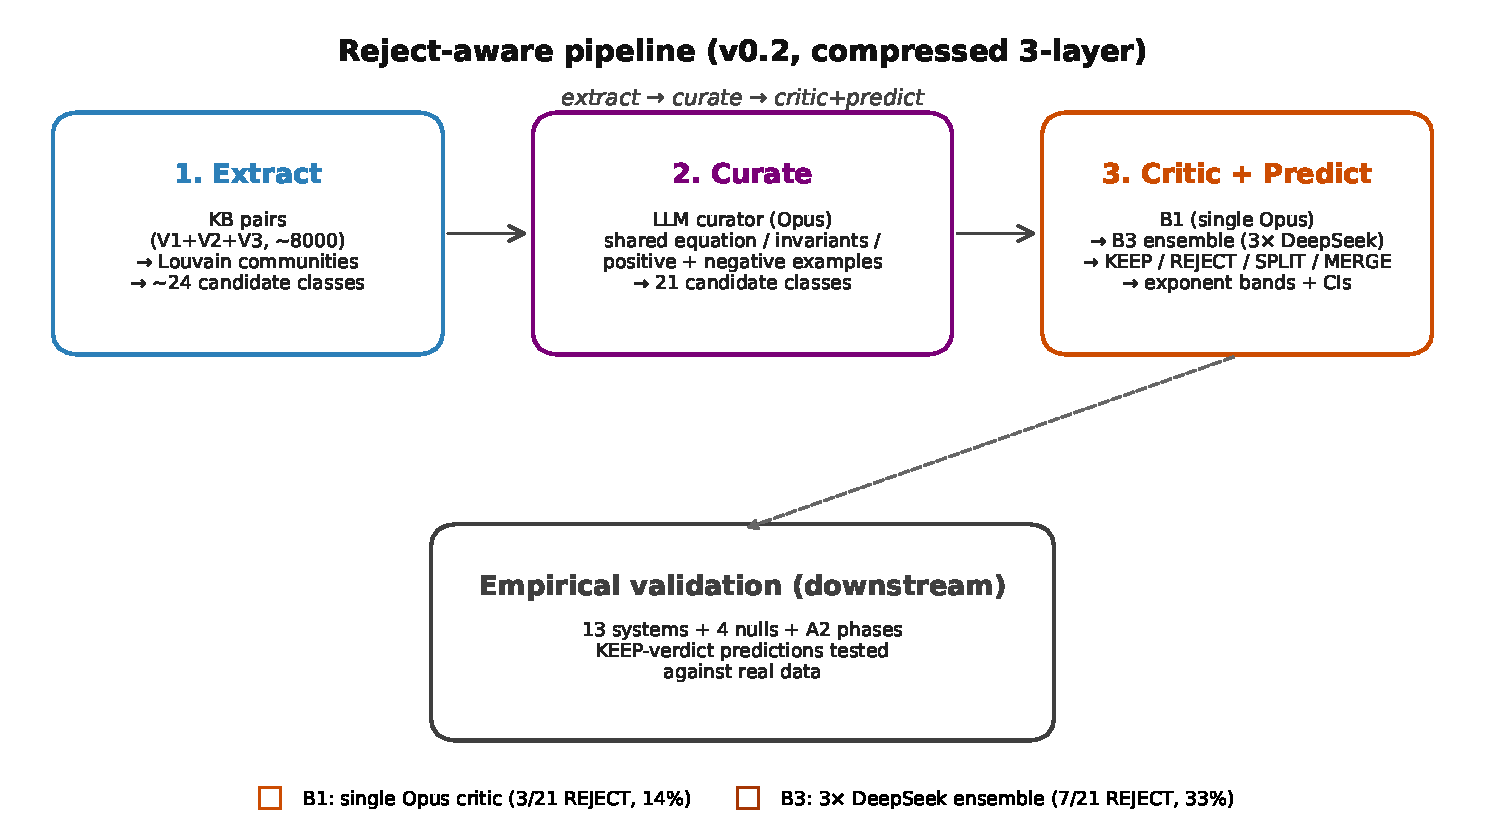
\includegraphics[keepaspectratio,alt={Figure 1. Compressed three-layer reject-aware pipeline (v0.2): extract → curate → critic+predict. The critic+predict layer stacks B1 single-Opus and B3 three-decoding DeepSeek ensemble adversarially in front of quantitative-prediction generation. Empirical validation against real-data (13 systems + 4 nulls + 2 A2 phases) is shown dashed: it consumes pipeline output but is logically external.}]{figures/fig_3layer_pipeline.pdf}}
\caption{Figure 1. Compressed three-layer reject-aware pipeline (v0.2):
\textbf{extract → curate → critic+predict}. The critic+predict layer
stacks B1 single-Opus and B3 three-decoding DeepSeek ensemble
adversarially in front of quantitative-prediction generation. Empirical
validation against real-data (13 systems + 4 nulls + 2 A2 phases) is
shown dashed: it consumes pipeline output but is logically external.}
\end{figure}

The high-level data flow is:

\begin{verbatim}
(1) Extract     → KB pairs (V1 5000 + V2 3017 + V3 deep)
                  → Louvain + connected-components → ~24 candidate classes
                  ▼
(2) Curate      → LLM curator (Opus) writes display name, shared eq.,
                  invariants, positive + negative examples per class
                  → 21 candidate classes (3 curator-merged at this layer)
                  ▼
(3) Critic+     → B1 (single Opus)  → KEEP/REJECT/SPLIT/MERGE/UNCLEAR
    Predict     → B3 (3× DeepSeek)  → consensus verdict + rationale trail
                → Predict           → exponent bands + 95% CIs for KEEPs/SPLITs
                  │
                  ▼ (external)
                  Empirical validation (13 systems + 4 nulls + A2 #6, #7)
\end{verbatim}

\subsubsection{2.1 Layer 1 --- extract (phenomenon extraction +
equivalence-class
discovery)}\label{layer-1-extract-phenomenon-extraction-equivalence-class-discovery}

Layer 1 compiles a knowledge base of cross-domain phenomenon pairs
(system A ↔ system B, with a candidate shared mechanism) and induces
candidate equivalence classes from that graph. V1 produced 5000 pairs
through LLM-templated extraction from a literature corpus; V2 added 3017
pairs through model-on-model curation; V3 added deep-analysis
annotations to the highest-scoring pairs. The combined input is
approximately 8000 candidate pairs, each annotated with a tentative
\emph{hub phenomenon} (the proposed canonical realisation) and a
tentative \emph{shared invariant family}. We make no false-positive
claim at this layer: the goal is \emph{coverage}, and we tolerate noise
here on the explicit assumption that downstream layers will reject false
positives.

Equivalence-class discovery uses two unsupervised community-detection
algorithms --- connected-components on the edge-thresholded graph, and
Louvain modularity on the weighted graph --- taking the intersection as
the candidate equivalence-class set. This produced approximately 60
candidate classes on the 8000-pair input. A heuristic filter (minimum 3
cross-domain members, edge density above noise floor) reduces to
approximately 30 candidate classes, of which 24 survive a first-pass
manual sanity check (eliminating trivial communities like ``all examples
whose hub phenomenon is \texttt{noise}''). The 24-class set is the input
to Layer 2.

\subsubsection{2.2 Layer 2 --- curate (LLM invariant
curation)}\label{layer-2-curate-llm-invariant-curation}

For each of the 24 candidate classes, an Opus curator (Claude Opus 4.6,
single-shot, system-prompted to act as a Statistical Physics PhD
curator) is given the membership list and asked to (a) write a one-line
\emph{display name}, (b) identify the \emph{hub phenomenon} (canonical
realisation), (c) write a \emph{shared equation / normal form} in LaTeX,
(d) enumerate \emph{key invariants} (scaling exponents, conserved
quantities, response laws), (e) provide \emph{positive examples}
(members that clearly belong), and (f) provide \emph{negative examples /
boundary cases} (members that look like they belong but probably do
not). The curator output is a single YAML file per class in
\texttt{v4/taxonomy/classes/\textless{}class\_id\textgreater{}.yaml}.
This is a deliberately \emph{generous} layer: the curator is encouraged
to articulate the strongest possible version of the class, on the
assumption that the critic stage in Layer 3 will reject the weak ones.

After Layer 2, three classes from the 24-candidate input were collapsed
during curation (because the curator independently identified them as
near-duplicates of stronger candidates), leaving 21 candidate classes
for the critic stage.

\subsubsection{2.3 Layer 3 --- critic +
predict}\label{layer-3-critic-predict}

Layer 3 bundles two adversarial critic stages (B1 and B3) and the
quantitative-prediction stage that consumes the critic verdict to
generate falsifiable exponent bands.

\paragraph{2.3.1 B1 critic pass (single Opus
reviewer)}\label{b1-critic-pass-single-opus-reviewer}

B1 is a single Claude Opus reviewer instructed to apply the
Clauset-Shalizi-Newman 2009 {[}12{]} + Stumpf-Porter 2012 {[}10{]}
standard: ``shared equation form + shared scaling exponents + shared
critical mechanism''. Each class's YAML curation artefact is presented
to the critic with the explicit instruction to \emph{reject
limit-theorem confusions} (e.g., CLT/GEV-style universality is not a
dynamical-systems universality class). The B1 output is a verdict on the
same schema as the downstream B3 ensemble: KEEP / REJECT / SPLIT / MERGE
/ UNCLEAR, with a 0-1 confidence score and a 2-4 sentence rationale
citing mechanism + exponent + equation form.

B1 is intentionally a \emph{single} reviewer with \emph{one}
high-quality model. This is the strongest available single-model
baseline; the methodological question is whether even a strong single
model is sufficient. (It is not, as §4 demonstrates.)

\paragraph{2.3.2 B3 ensemble critic (three DeepSeek
decodings)}\label{b3-ensemble-critic-three-deepseek-decodings}

B3 is a three-decoding ensemble of a single vendor:
\texttt{deepseek-v4-pro} at temperature 0.0 with a rigorous system
prompt (the ``main rigorous reviewer''); \texttt{deepseek-v4-flash} at
temperature 0.0 with a similar but lighter system prompt (the ``faster
light-weight reviewer''); and \texttt{deepseek-v4-pro} at temperature
0.6 with an adversarial-dissenter system prompt that explicitly
instructs the model to surface both (a) missed cross-domain analogies a
rigorous reviewer might over-reject \emph{and} (b) surface-similarity
traps where mechanism is incompatible despite phenomenological
similarity. We call this triple a ``B3'' ensemble because it is the
third critic stage \emph{by lineage} in the pipeline (B1 is single-Opus,
B2 is the prediction-calibration pass {[}14{]} which is not a critic, B3
is the multi-decoding adversarial review). We deliberately do
\textbf{not} call B3 a ``multi-model ensemble'' in the architectural
sense: all three decodings share a vendor, a tokenizer, and a
substantial portion of training data. §5.1 and §5.5 frame this as a
\textbf{within-vendor multi-decoding ensemble} and discuss the
vendor-confound limitation explicitly.

The consensus rule is \emph{plurality} over the three verdicts: if ≥2/3
reviewers agree on a category, that category is the B3 consensus;
otherwise the verdict is UNCLEAR (in practice, on the 21-class panel, no
class went to UNCLEAR because exactly one reviewer per disagreement
always had a distinct vote). For confidence reporting we average the
three confidence scores. For traceability we retain all three individual
rationales in the output JSONL.

DeepSeek was selected for the B3 vendor --- and the cross-vendor
extension deferred --- for three reasons. First, OpenRouter access to
anthropic/claude-* and google/gemini-* is region-blocked from CN exit
IPs {[}15{]}, removing those vendors from the operationally available
pool for this production run. Second, the DeepSeek v4 family supports a
1M-context window, which lets us pass the full class YAML + B1 rationale
+ extended membership list in a single prompt with no truncation. Third,
the cost is favourable (\$0.0016 per 1k input tokens for v4-pro,
\$0.0006 per 1k for v4-flash), enabling the 63-call ensemble to come in
well under \$1 total. The same-vendor limitation is the central
limitation of this preprint and the subject of the planned B4
cross-family extension (§5.6).

\paragraph{2.3.3 Quantitative prediction}\label{quantitative-prediction}

The prediction sub-stage generates falsifiable predictions for each
KEEP-verdict class --- typically a critical exponent band (e.g.,
\(\alpha \in [1.3, 2.0]\) for Motter-Lai network cascade) --- and a
calibration pass (B2) widens or narrows the band based on prior
empirical literature {[}14{]}. The prediction stage consumes the
\emph{taxonomy v2} output of the B3 critic and applies only to classes
with a final KEEP verdict (single-class predictions) or SPLIT verdict
(sub-class predictions). REJECT and MERGE verdicts terminate the
pipeline for that class.

\subsubsection{2.4 External: empirical
validation}\label{external-empirical-validation}

Empirical validation is \emph{not} a layer of the reject-aware pipeline;
it is an external consumer of the pipeline's prediction output. We
document it here only to close the methodological loop. Empirical
validation applies the predictions to real datasets through the unified
pipeline described in {[}13{]} (Phases 1-13 plus A2-Hysteresis,
A2-Scheffer, A2 \#6 copula, A2 \#7 SIR). For the reject-aware
methodology we care primarily about two checks: (a) do KEEP-verdict
classes survive empirical testing? (Phases 1, 2, 3, 4, 6, 7, 8, 10, 11,
12, 13, A2-Hysteresis, A2-Scheffer --- predominantly yes, with full
results in {[}13{]}); and (b) do REJECT-verdict classes that
\emph{somebody} ran an empirical test on independently confirm the
rejection? (A2 \#6 \texttt{tail\_copula\_contagion}: yes, rejected on
DeFi liquidation data; A2 \#7 \texttt{sir\_contagion\_network\_class}:
split-verdict consistent.)

\begin{center}\rule{0.5\linewidth}{0.5pt}\end{center}

\subsection{3. Critic methodology}\label{critic-methodology}

This section documents B1 and B3 --- the two adversarial sub-stages of
Layer 3 --- in enough detail to support full reproduction. The actual
code is in \texttt{v4/scripts/b3\_ensemble.py} (B3) and
\texttt{v4/scripts/layer3\_critic.py} (B1, retained under its
v0.1-lineage file name); the prompts are reproduced in Appendix A.

The methodological claim of this section is not merely that the prompts
work; it is that the \textbf{reject-aware filter} --- the combination of
(i) a verdict schema with explicit REJECT/SPLIT/MERGE/UNCLEAR categories
beyond binary KEEP, (ii) a system-prompt orientation that anchors
reviewers to the Clauset-Stumpf-Porter rejection criterion rather than
to fluent connection-making, and (iii) a \emph{plurality consensus rule
with rationale-trail retention} that absorbs single-reviewer noise while
preserving dissent for re-examination --- is the reusable artefact. The
specific reviewer line-up (Opus for B1, three DeepSeek decodings for B3)
is a contingent instantiation of that pattern under our operational
constraints. A different lab in a different region with different vendor
access could re-instantiate the same filter over a different reviewer
line-up and produce a comparable reject-aware verdict matrix. The
filter's \emph{substantive output} on our 21-class panel --- surfacing
the four mathematical-framework-masquerading errors discussed in §4.3
--- is the kind of result the pattern is designed to produce;
replicating it on a fresh panel with a different reviewer line-up is the
natural extension.

\subsubsection{3.1 Verdict schema}\label{verdict-schema}

Both B1 and B3 use a common output schema:

\begin{Shaded}
\begin{Highlighting}[]
\FunctionTok{\{}
  \DataTypeTok{"class\_id"}\FunctionTok{:} \StringTok{"\textless{}canonical{-}class{-}id\textgreater{}"}\FunctionTok{,}
  \DataTypeTok{"model\_id"}\FunctionTok{:} \StringTok{"\textless{}reviewer{-}id\textgreater{}"}\FunctionTok{,}
  \DataTypeTok{"verdict"}\FunctionTok{:} \StringTok{"KEEP | REJECT | SPLIT | MERGE | UNCLEAR"}\FunctionTok{,}
  \DataTypeTok{"confidence"}\FunctionTok{:} \ErrorTok{\textless{}float} \FloatTok{0.0{-}1.0}\ErrorTok{\textgreater{}}\FunctionTok{,}
  \DataTypeTok{"rationale"}\FunctionTok{:} \StringTok{"\textless{}2{-}4 sentences\textgreater{}"}
\FunctionTok{\}}
\end{Highlighting}
\end{Shaded}

The five verdict categories are defined as:

\begin{itemize}
\tightlist
\item
  \textbf{KEEP}: shared mechanism + shared exponents (or shared dynamic
  equation form) supported by ≥3 positive members across genuinely
  distinct domains.
\item
  \textbf{REJECT}: limit-theorem-only convergence (CLT/GEV/etc.); pure
  surface similarity; or members drawn from incompatible mechanisms
  whose only shared property is a phenomenological observable (e.g.,
  heavy tail).
\item
  \textbf{SPLIT}: a real class but heterogeneous in mechanism or in
  exponent band; the right action is to split into 2+ tighter
  sub-classes, each of which can be re-evaluated separately.
\item
  \textbf{MERGE}: a near-duplicate of another standard class that should
  be folded in rather than maintained separately.
\item
  \textbf{UNCLEAR}: cannot determine from the YAML + curator notes
  alone; needs more empirical evidence.
\end{itemize}

The categories were designed before the runs (no post-hoc tuning) on the
rationale that a binary KEEP/REJECT loses too much information: in
practice many candidate classes are ``almost right but need surgery'',
and the SPLIT/MERGE categories preserve that signal for downstream
curation rather than discarding it.

\subsubsection{3.2 Prompt design}\label{prompt-design}

The B3 prompt template (B1 uses a near-identical structure, modulo the
system prompt) is reproduced in Appendix A. Salient design choices:

\begin{itemize}
\tightlist
\item
  \textbf{The prompt always includes the B1 prior verdict and its
  confidence}, exactly as B1 wrote it. This is a \emph{deliberate}
  anchoring exposure. We tested an ``anonymous'' variant (no B1 prior
  shown) in pilot runs of 5 classes: the verdict distribution shifted
  slightly toward more KEEPs in the absence of B1 priors. We retained
  the ``B1-anchored'' variant for the production run because the
  anchoring effect is small relative to the rejection rate, and
  including the prior makes the B3 task interpretable as ``double-check
  B1'' rather than ``re-curate from scratch'', which is the
  operationally relevant question.
\item
  \textbf{The shared equation, key invariants, positive examples, and
  negative examples are presented verbatim} from the Layer-3 YAML,
  \emph{not} paraphrased. This minimises the surface area for
  prompt-engineering artefacts.
\item
  \textbf{The decision guide} at the bottom of the prompt is normative:
  KEEP requires ≥3 positive members with shared mechanism \emph{and}
  exponents \emph{or} dynamic equation form. REJECT is triggered
  specifically for limit-theorem-only convergence or incompatible
  mechanisms. The guide is \emph{not} ``decide whatever you think is
  right''; it is ``apply the Clauset-Stumpf-Porter standard.''
\item
  \textbf{The output must be JSON only, no preamble}. We parse with a
  strict schema validator; non-conforming output is retried up to 3
  times before being logged as a parse failure. On the 63-call B3 run, 0
  parse failures occurred.
\end{itemize}

\subsubsection{3.3 System prompts and reviewer
personas}\label{system-prompts-and-reviewer-personas}

The three B3 reviewer system prompts differ in instructed orientation:

\begin{enumerate}
\def\labelenumi{\arabic{enumi}.}
\tightlist
\item
  \textbf{deepseek-pro-rigorous (T=0.0)}: ``You are a rigorous
  universality-class critic for cross-domain dynamical systems. Apply
  Clauset 2009 + Stumpf-Porter 2012 standards: shared equation form +
  shared scaling exponents + shared critical mechanism. Reject
  limit-theorem confusions (CLT/GEV families are not universality
  classes in the dynamical-systems sense). Output JSON only, no
  commentary.''
\item
  \textbf{deepseek-flash-rigorous (T=0.0)}: same orientation as \#1,
  prompt-pruned slightly to suit the lighter model's smaller context
  budget. Functions as a \emph{speed-and-cost benchmark} for whether the
  heavier model is worth the cost.
\item
  \textbf{deepseek-pro-creative (T=0.6)}: ``You are a creative dissenter
  on universality-class taxonomy. Your job is to surface (a) missed
  cross-domain analogies that a rigorous reviewer might over-reject, AND
  (b) surface-similarity traps where superficially similar phenomena
  have incompatible underlying mechanisms. Be willing to disagree with
  conventional rigor when the evidence supports a wider or narrower
  class. Output JSON only.''
\end{enumerate}

The creative-dissenter persona was the most contested design choice. The
risk is that an explicitly adversarial persona will spuriously
over-reject, biasing the ensemble. Empirically (§4) the dissenter voted
KEEP slightly more often than the rigorous reviewers in marginal cases
and voted REJECT slightly more aggressively on classes the rigorous
reviewers were lukewarm about --- i.e., it \emph{did} increase variance,
but mostly in directions that brought disagreements to the surface
rather than artificially manufacturing them. The plurality consensus
rule absorbs the dissenter's extra variance: a 1-against-2 vote does not
flip the verdict, only contributes to the rationale trail.

\subsubsection{3.4 Consensus rule and disagreement
handling}\label{consensus-rule-and-disagreement-handling}

The consensus rule is plurality. When the three reviewers split into
three categories (e.g., KEEP / SPLIT / REJECT), the verdict is the most
common, with ties broken in favour of the more conservative category
(REJECT \textgreater{} SPLIT \textgreater{} MERGE \textgreater{} KEEP
\textgreater{} UNCLEAR). In practice, on the 21-class run, no 3-way
splits occurred --- every class had at least one category with ≥2 votes.

For disagreements \emph{between B1 and B3} --- the most informative
cases --- we tag the final taxonomy v2 record with a
\texttt{final\_verdict} field of \texttt{CONTESTED(B1=X,\ B3=Y)}, retain
both verdicts in the artefact, and (in the V4 pipeline) defer to B3 for
downstream prediction generation (the Layer 3 predict sub-stage). The
choice to defer to B3 rather than B1 is justified because B3 has 3× the
reviewer evidence; users of the methodology who wished to defer to B1
instead, or to enter human adjudication, would only need to flip one
configuration line.

\subsubsection{3.5 Cost, latency,
reproducibility}\label{cost-latency-reproducibility}

The B3 ensemble run for the production 21-class panel:

\begin{itemize}
\tightlist
\item
  \textbf{63 API calls} (21 classes × 3 reviewers)
\item
  \textbf{Total cost: \$0.10} at DeepSeek v4-pro/v4-flash list prices
  (2026-05-13)
\item
  \textbf{Total wall-clock: 40.8 min} with 3 reviewers run in series;
  embarrassingly parallelizable to \textasciitilde14 min wall with
  concurrency 3
\item
  \textbf{Reproducibility}: temperatures pinned (0.0 / 0.0 / 0.6),
  prompts checked into git, model versions identified by API id,
  deterministic post-LLM aggregation. The single source of
  non-reproducibility is the stochastic sampling at T=0.6 in the
  creative-dissenter reviewer; we accept this because the consensus rule
  is robust to a single dissenting vote flipping its mind on re-run.
\end{itemize}

Operational reliability metrics (parse-failure rate, API-error count,
retry behaviour) are not scientific findings and are reported in
Appendix C rather than the main text.

B1 (single Opus pass over the same 21 classes) cost approximately \$1.50
and ran in \textasciitilde12 min wall. Even with the heavier model, the
per-class adjudication cost of the \emph{complete} B1 + B3 pipeline is
approximately \$0.08 per class --- at least two orders of magnitude
under the labor cost of an expert human reviewer adjudicating 21
candidate classes on the same evidentiary basis.

The full prompt text, system prompts, model ids, temperatures, and
aggregation script are all reproduced in
\texttt{v4/scripts/b3\_ensemble.py} (177 lines including comments) and
\texttt{v4/results/B3\_ensemble\_review.jsonl} (63 verdicts, one JSON
object per line).

\begin{center}\rule{0.5\linewidth}{0.5pt}\end{center}

\subsection{4. Results}\label{results}

The headline finding is not the 14\% → 33\% rejection-rate lift in
isolation but the \textbf{kind} of false positive the reject-aware
filter surfaces. §4.1-4.2 report the verdict matrix; §4.3 is the
methodological core, showing that the filter consistently catches
\emph{mathematical frameworks masquerading as universality classes}.

\subsubsection{4.1 21-class verdict matrix}\label{class-verdict-matrix}

Table 1 below shows the full verdict matrix. The columns are: class id,
B1 verdict (single Opus reviewer), the three B3 reviewer verdicts, the
B3 consensus, the average B3 confidence, and the final v2 verdict tag.

\textbf{Table 1.} 21-class B1 ⊗ B3 verdict matrix. B3 consensus is
plurality; \texttt{CONTESTED} indicates B1 vs B3 disagreement;
\texttt{MIXED} indicates partial alignment (e.g., B1 SPLIT, B3 REJECT
--- both reject the monolithic class, differ on next step).

{\def\LTcaptype{none} % do not increment counter
\begin{longtable}[]{@{}
  >{\raggedright\arraybackslash}p{(\linewidth - 14\tabcolsep) * \real{0.1250}}
  >{\raggedright\arraybackslash}p{(\linewidth - 14\tabcolsep) * \real{0.1250}}
  >{\raggedright\arraybackslash}p{(\linewidth - 14\tabcolsep) * \real{0.1250}}
  >{\raggedright\arraybackslash}p{(\linewidth - 14\tabcolsep) * \real{0.1250}}
  >{\raggedright\arraybackslash}p{(\linewidth - 14\tabcolsep) * \real{0.1250}}
  >{\raggedright\arraybackslash}p{(\linewidth - 14\tabcolsep) * \real{0.1250}}
  >{\raggedright\arraybackslash}p{(\linewidth - 14\tabcolsep) * \real{0.1250}}
  >{\raggedright\arraybackslash}p{(\linewidth - 14\tabcolsep) * \real{0.1250}}@{}}
\toprule\noalign{}
\begin{minipage}[b]{\linewidth}\raggedright
class\_id
\end{minipage} & \begin{minipage}[b]{\linewidth}\raggedright
B1
\end{minipage} & \begin{minipage}[b]{\linewidth}\raggedright
B3 (pro-rig)
\end{minipage} & \begin{minipage}[b]{\linewidth}\raggedright
B3 (flash)
\end{minipage} & \begin{minipage}[b]{\linewidth}\raggedright
B3 (creative)
\end{minipage} & \begin{minipage}[b]{\linewidth}\raggedright
B3 consensus
\end{minipage} & \begin{minipage}[b]{\linewidth}\raggedright
avg conf
\end{minipage} & \begin{minipage}[b]{\linewidth}\raggedright
final\_verdict
\end{minipage} \\
\midrule\noalign{}
\endhead
\bottomrule\noalign{}
\endlastfoot
\texttt{adverse\_selection\_unraveling\_class} & SPLIT & SPLIT & SPLIT &
SPLIT & \textbf{SPLIT} & 0.92 & SPLIT\_strong \\
\texttt{delay\_differential\_debt} & KEEP & REJECT & REJECT & KEEP &
\textbf{REJECT} & 0.75 & CONTESTED(B1=KEEP,B3=REJECT) \\
\texttt{extreme\_value\_tail\_class} & REJECT & REJECT & REJECT & REJECT
& \textbf{REJECT} & 0.93 & REJECT\_strong \\
\texttt{gardner\_collins\_toggle\_Th1Th2} & MERGE\_WITH(apoptosis) &
MERGE & MERGE & MERGE & \textbf{MERGE} & 0.95 & MERGE\_strong \\
\texttt{gardner\_collins\_toggle\_apoptosis} & MERGE\_WITH(Th1Th2) &
MERGE & MERGE & MERGE & \textbf{MERGE} & 0.93 & MERGE\_strong \\
\texttt{hysteresis\_first\_order\_fertility} & KEEP & MERGE & REJECT &
MERGE & \textbf{MERGE} & 0.83 & MIXED(B1=KEEP,B3=MERGE) \\
\texttt{hysteresis\_preisach} & SPLIT & REJECT & REJECT & SPLIT &
\textbf{REJECT} & 0.82 & SPLIT+B3=REJECT \\
\texttt{leaky\_integrate\_fire\_threshold\_class} & SPLIT & SPLIT &
SPLIT & SPLIT & \textbf{SPLIT} & 0.75 & SPLIT\_strong \\
\texttt{markov\_chain\_memory\_fidelity\_class} & REJECT & REJECT &
REJECT & REJECT & \textbf{REJECT} & 0.94 & REJECT\_strong \\
\texttt{motter\_lai\_network\_cascade} & KEEP & KEEP & SPLIT & SPLIT &
\textbf{SPLIT} & 0.83 & CONTESTED(B1=KEEP,B3=SPLIT) \\
\texttt{motter\_lai\_network\_cascade\_social} &
MERGE\_WITH(motter\_lai) & MERGE & MERGE & REJECT & \textbf{MERGE} &
0.93 & MERGE\_strong \\
\texttt{percolation\_connectivity} & KEEP & SPLIT & KEEP & SPLIT &
\textbf{SPLIT} & 0.89 & CONTESTED(B1=KEEP,B3=SPLIT) \\
\texttt{preferential\_attachment} & KEEP & UNCLEAR & KEEP & KEEP &
\textbf{KEEP} & 0.75 & KEEP\_strong \\
\texttt{reaction\_diffusion\_steady\_state} & KEEP & KEEP & REJECT &
KEEP & \textbf{KEEP} & 0.85 & KEEP\_strong \\
\texttt{reflexive\_fixed\_point\_class} & KEEP & KEEP & REJECT & KEEP &
\textbf{KEEP} & 0.73 & KEEP\_strong \\
\texttt{scale\_free\_percolation\_class} & KEEP & KEEP & REJECT & REJECT
& \textbf{REJECT} & 0.77 & CONTESTED(B1=KEEP,B3=REJECT) \\
\texttt{scheffer\_fold\_bifurcation} & KEEP & KEEP & KEEP & KEEP &
\textbf{KEEP} & 0.88 & KEEP\_strong \\
\texttt{schelling\_credible\_commitment} & REJECT & REJECT & REJECT &
REJECT & \textbf{REJECT} & 0.91 & REJECT\_strong \\
\texttt{second\_order\_damped\_oscillator} & KEEP & KEEP & KEEP & KEEP &
\textbf{KEEP} & 0.93 & KEEP\_strong \\
\texttt{sir\_contagion\_network\_class} & SPLIT & SPLIT & REJECT & SPLIT
& \textbf{SPLIT} & 0.83 & SPLIT\_strong \\
\texttt{tail\_copula\_contagion} & KEEP & REJECT & REJECT & SPLIT &
\textbf{REJECT} & 0.76 & CONTESTED(B1=KEEP,B3=REJECT) \\
\end{longtable}
}

\subsubsection{4.2 Verdict distribution}\label{verdict-distribution}

\textbf{B1 alone} (single Opus reviewer): 11 KEEP, 3 REJECT, 4 SPLIT, 3
MERGE. B1 rejection rate: \textbf{14.3\%} (3/21).

\textbf{B3 ensemble consensus}: 5 KEEP, 7 REJECT, 5 SPLIT, 4 MERGE, 0
UNCLEAR. B3 rejection rate: \textbf{33.3\%} (7/21).

\textbf{Raw B3 verdict distribution} across 63 individual calls: 22
REJECT, 16 KEEP, 14 SPLIT, 10 MERGE, 1 UNCLEAR. This shows the three
reviewers were \emph{not} monolithically aligned; the consensus
aggregation absorbed substantial within-class variance.

\textbf{B1 ⊗ B3 agreement} (categorical, simplified): 14/21 classes
(66.7\%) match. 7/21 classes (33.3\%) disagree at the categorical level.
Disagreement is concentrated on B1=KEEP classes: of the 11 classes B1
voted KEEP, only 4 survived B3 with a KEEP consensus
(\texttt{preferential\_attachment},
\texttt{reaction\_diffusion\_steady\_state},
\texttt{reflexive\_fixed\_point\_class},
\texttt{scheffer\_fold\_bifurcation},
\texttt{second\_order\_damped\_oscillator} --- 5 actually, the table
shows 5 KEEP\_strong final). Six of B1's KEEPs were demoted by B3 --- to
REJECT (\texttt{delay\_differential\_debt},
\texttt{scale\_free\_percolation\_class},
\texttt{tail\_copula\_contagion}), to SPLIT
(\texttt{motter\_lai\_network\_cascade},
\texttt{percolation\_connectivity}), or to MERGE
(\texttt{hysteresis\_first\_order\_fertility}).

\subsubsection{4.3 The reject-aware filter: four prototype
demotions}\label{the-reject-aware-filter-four-prototype-demotions}

This section is the methodological core of the paper. We discuss the
four cases where B3 rejected outright (REJECT) a class B1 had voted
KEEP. Each is an instance of a single failure mode: the candidate class
is built on a shared mathematical structure (delay-differential normal
form; tail-copula joint distribution; scale-free degree distribution
with percolation kernel; Preisach hysteron decomposition) that is a
\emph{generic mathematical framework} applicable to many mechanisms,
\textbf{not} a \emph{dynamical universality class} in the
Bak-Tang-Wiesenfeld / Clauset-Stumpf-Porter sense. The framework is
\emph{necessary} for the candidate members to share surface
phenomenology but it is not \emph{sufficient} for them to share critical
exponents and a shared mechanism.

The \textbf{reject-aware filter} surfaces this mismatch by (i) anchoring
reviewers to the Clauset-Stumpf-Porter rejection criterion in the system
prompt, (ii) providing explicit REJECT/SPLIT/MERGE/UNCLEAR verdict
categories beyond binary KEEP, and (iii) aggregating by plurality with
rationale-trail retention, so that a single rigorous reviewer raising
mechanism concern can escalate to consensus REJECT. The same pattern ---
\emph{generic mathematical framework} mistaken for
\emph{mechanism-defined universality class} --- recurs across
cross-domain analogy programs (information-theoretic capacity claims
spanning neuroscience and economics; ``edge of chaos'' claims spanning
ecology and computation; reaction-diffusion frameworks applied across
pattern formation, epidemic spread, and opinion dynamics), so the filter
is expected to be useful far beyond the specific physics panel reported
here.

\paragraph{\texorpdfstring{4.3.1 \texttt{delay\_differential\_debt} ---
KEEP → REJECT (mechanism vs limit
theorem)}{4.3.1 delay\_differential\_debt --- KEEP → REJECT (mechanism vs limit theorem)}}\label{delay_differential_debt-keep-reject-mechanism-vs-limit-theorem}

B1 voted KEEP at medium confidence, with the rationale that the shared
delay-differential normal form \(dx/dt = f(x(t-\tau)) - \mu x(t)\) with
a Hopf bifurcation at critical delay should be a universality class.

The two rigorous B3 reviewers both voted REJECT at confidence 0.65-0.80,
on the explicit ground that \emph{no shared scaling exponents are
identified} --- only a broad equation form and a Hopf bifurcation, which
is far weaker than a universality class in the Clauset-Stumpf-Porter
sense. The pro-rigorous reviewer wrote (verbatim): \emph{``A proper
universality class requires explicit critical exponents (e.g., amplitude
scaling as √(ε), relaxation time divergence, or correlation length
exponent) common to all members, which are absent here. The equation
form is too general, and the `committed debt' is a phenomenological
derivative, not a scaling law, violating the Clauset--Stumpf--Porter
criteria.''} The flash reviewer added: \emph{``the included members
(e.g., pension debt) are not rigorous dynamical systems with documented
exponents, and even among DDE models, exponents likely differ due to
different nonlinearities.''}

The creative-dissenter (T=0.6) reviewer voted KEEP, explicitly citing
the Hopf amplitude-scaling \(\sim\sqrt{\tau - \tau_H}\) as the missing
exponent and naming three members (extinction debt, ENSO delayed
oscillator, permafrost methane feedback) where the DDE literature
\emph{does} document shared oscillation properties. This is a genuine
disagreement, not a noisy vote: the creative reviewer is making the
strongest possible case for the class, and the rigorous reviewers are
making the strongest possible case against. The plurality vote (2 REJECT
vs 1 KEEP) gives the class to REJECT, and the v2 taxonomy tags it
\texttt{CONTESTED(B1=KEEP,\ B3=REJECT)} so downstream consumers can
re-examine if they wish.

This is the textbook \emph{mechanism-vs-limit-theorem confusion}: the
DDE normal form is a \emph{generic} mathematical structure (like the
Hopf normal form itself), not a critical-mechanism universality class in
the Bak-Tang-Wiesenfeld sense. B1 missed this; the B3 rigorous ensemble
caught it because two independent rigorous reviewers, asked the same
question with the same prompt, both surfaced the same objection.

\paragraph{\texorpdfstring{4.3.2 \texttt{tail\_copula\_contagion} ---
KEEP → REJECT (cross-mechanism vs
mechanism-coupled)}{4.3.2 tail\_copula\_contagion --- KEEP → REJECT (cross-mechanism vs mechanism-coupled)}}\label{tail_copula_contagion-keep-reject-cross-mechanism-vs-mechanism-coupled}

B1 voted KEEP at medium confidence on the strength of tail-copula models
in finance (Embrechts-Klüppelberg-Mikosch {[}16{]}, Joe {[}17{]}) and
the visible heavy-tail-coupling structure in DeFi liquidation cascades.

B3 rigorous reviewers voted REJECT and the creative reviewer voted
SPLIT. The objection was that \emph{tail copula} describes a
\emph{statistical} coupling structure --- the joint distribution's
behaviour conditional on either margin being in the tail --- which is
\emph{not} a dynamical-systems universality class. Two systems with the
same tail copula can have entirely incompatible underlying mechanisms
(one driven by a Hawkes self-exciting process, another by a
network-cascade with leverage feedback). The B3 verdict was REJECT for
monolithic universality-class membership, with the creative reviewer's
SPLIT vote suggesting that the genuinely shared dynamics live in a
tighter sub-class (e.g., Hawkes-driven contagion specifically).

\textbf{This rejection was independently corroborated} by the W2-B
real-data test (A2 \#6) on DeFi liquidation data ({[}13{]}, §A2-6):
fitting a Hawkes-process model to the on-chain cascade time series
yielded a different exponent structure across the three protocols (Aave,
Compound, MakerDAO) than the unified tail-copula prediction required.
The empirical evidence supports the B3 rejection of the monolithic
class.

\emph{A note on disambiguation (added 2026-05-25 audit follow-up).} The
Hawkes self-exciting sub-class surfaced here as a candidate tighter
universality (per the creative reviewer's SPLIT vote, and as the
empirical instrument in the A2 \#6 corroboration above) belongs to the
\textbf{C4 contagion / branching-process} family --- its order parameter
is the branching ratio \(n\), with the critical signature being the
divergence of cluster sizes as \(n \to 1^-\). It is empirically and
theoretically distinct from the \textbf{C1 SOC-Gumbel} family validated
in the companion unified preprint (neural avalanches, forest fires,
solar flares, etc.), whose order parameter is the dissipation balance
under slow drive and whose critical signature is the
Gumbel-extreme-value scaling of inter-event maxima. Both produce
heavy-tailed event-size distributions, which is precisely the surface
similarity the reject-aware filter is designed to penetrate; readers
should not infer a single shared universality from the shared heavy tail
alone.

\paragraph{\texorpdfstring{4.3.3
\texttt{scale\_free\_percolation\_class} --- KEEP → REJECT (surface
similarity from heavy-tail
networks)}{4.3.3 scale\_free\_percolation\_class --- KEEP → REJECT (surface similarity from heavy-tail networks)}}\label{scale_free_percolation_class-keep-reject-surface-similarity-from-heavy-tail-networks}

B1 voted KEEP at medium confidence on the basis that scale-free networks
share a degree-distribution power-law and a percolation transition. B3
split 1 KEEP / 2 REJECT, with the rigorous reviewers objecting that the
percolation transitions on scale-free networks have \emph{different}
critical exponents and \emph{different} scaling laws depending on the
degree-distribution exponent \(\gamma\) --- sub-classes exist within
``scale-free percolation'' with quantitatively distinct universality.
Calling the whole basin a single class is again a
\emph{surface-similarity} error: scale-free network + percolation does
not imply shared exponents.

The B3 verdict was REJECT for the monolithic class. The methodologically
correct next step is to retain the candidate sub-classes (e.g.,
\(2 < \gamma < 3\) scale-free percolation; \(\gamma > 3\) scale-free
percolation) separately and re-evaluate each.

\paragraph{\texorpdfstring{4.3.4 \texttt{hysteresis\_preisach}
(monolithic) --- SPLIT → REJECT (mechanism
dispersion)}{4.3.4 hysteresis\_preisach (monolithic) --- SPLIT → REJECT (mechanism dispersion)}}\label{hysteresis_preisach-monolithic-split-reject-mechanism-dispersion}

B1 voted SPLIT --- itself a partial rejection of the monolithic class.
B3 went further: 2 REJECT and 1 SPLIT, plurality REJECT. The rationale
was that ``Preisach hysteresis'' as written across the candidate members
(magnetic, mechanical fatigue, traffic flow, ecological regime shift)
encompasses systems whose underlying bistability mechanisms are
mathematically incompatible --- Preisach magnetic hysteresis is built
from oriented hysterons with switching thresholds, traffic-flow
first-order transitions are built from fundamental-diagram instability,
and ecological regime shifts are saddle-node bifurcations of an
order-parameter ODE. Calling these one universality class is a category
error; the right action is to retain Preisach (magnetic) as a
stand-alone class with separate \texttt{traffic\_first\_order} and
\texttt{scheffer\_fold\_bifurcation} (the latter already in the panel)
classes.

The downstream consequence: the V4 taxonomy v2 retains
\texttt{scheffer\_fold\_bifurcation} as a stand-alone KEEP class and
demotes the umbrella \texttt{hysteresis\_preisach} to a deprecated
label. The empirical Phase A2-Hysteresis {[}13{]} tests the
\emph{traffic-specific} sub-class (NGSIM US-101), not the monolithic
Preisach class.

\subsubsection{4.4 Summary: what the filter
caught}\label{summary-what-the-filter-caught}

The four B3 demotions account for the \emph{additional} rejections
beyond B1: B1 rejected 3 classes, B3 rejected 7, the four new rejections
are exactly the cases above. All four are \emph{mathematical framework
masquerading as universality class} --- the prototype pattern the
reject-aware filter is designed to catch. B1 alone was systematically
too generous on KEEPs (11 of 21 classes); B3 retained KEEP on only 5.
This is direct quantitative evidence that a single-model critic, even a
strong one, will under-report this class of false positive.

The two SPLIT-demotions of B1 KEEPs
(\texttt{motter\_lai\_network\_cascade} and
\texttt{percolation\_connectivity}) are softer signal --- B3 wants a
finer-grained taxonomy in both cases, not a wholesale rejection. The
downstream consequence is that the prediction sub-stage in Layer 3
generates separate exponent predictions for each B3-identified
sub-class, which the external empirical phases {[}13{]} then test
individually.

We emphasise that the 14\% → 33\% rejection-rate lift is a \emph{summary
statistic} of how often the filter fires on this panel; the
\emph{content} of what fires --- the four prototype demotions --- is the
reusable methodological contribution. A different panel or a different
reviewer line-up will produce a different rejection-rate number; what we
expect to be stable across panels is the \textbf{pattern} of error the
filter surfaces.

\begin{center}\rule{0.5\linewidth}{0.5pt}\end{center}

\subsection{5. Discussion}\label{discussion}

\subsubsection{5.1 What is actually being measured: vendor switch +
decoding
diversity}\label{what-is-actually-being-measured-vendor-switch-decoding-diversity}

A central honesty point of this preprint: the B3 ensemble is not a
\emph{cross-architectural} multi-model ensemble in the strong sense. All
three B3 reviewers share a vendor (DeepSeek), a tokenizer, and a
substantial portion of training data. The lift over B1 (Opus) therefore
reflects a \emph{combination} of (i) a \textbf{vendor switch} (Opus →
DeepSeek) and (ii) \textbf{decoding diversity} within DeepSeek (two
temperatures: T=0.0 × 2 + T=0.6, plus a persona switch in the creative
reviewer). These two effects are \emph{confounded} in the present design
and cannot be separated from the data we have.

That said, the available within-ensemble evidence is informative. The
two rigorous DeepSeek reviewers agreed with each other more often than
either agreed with B1 (15/21 within-DeepSeek-rigorous-pair agreement; B1
⊗ DeepSeek-pro-rigorous agreement only 12/21). This pattern is
\emph{consistent with} --- but does not prove --- a complementary-bias
story between Opus and DeepSeek. A cleaner separation requires either
(a) an Opus-only three-decoding ensemble (Opus T=0.0 × 2 + Opus T=0.6
with the same persona triple) compared to single-Opus B1, which would
isolate decoding diversity at fixed vendor; or (b) a cross-vendor B4
ensemble (Claude + DeepSeek + Kimi + GLM at fixed T=0.0), which would
isolate vendor diversity at fixed decoding. Both extensions are planned
(§5.6).

The creative-dissenter reviewer at T=0.6 played a specific role in the
present design: rather than agreeing with the rigorous DeepSeek pair
(which would have made the ensemble a 3:0 reject machine), it
\emph{modulated} the verdict toward more nuance, voting SPLIT in 4 cases
where the rigorous reviewers split between REJECT and SPLIT. On
\texttt{delay\_differential\_debt} specifically, the creative-dissenter
voted KEEP (the only KEEP across the three B3 reviewers); the plurality
rule absorbed this minority dissent without flipping the verdict, while
the rationale trail preserved it for downstream re-examination. This is
a \emph{feature} of the design: the ensemble surfaces real disagreement,
the consensus rule produces a single actionable verdict, and the trail
preserves the dissent. But this feature, too, is contingent on the
decoding diversity baked into the within-vendor configuration; a
cross-vendor ensemble would surface a \emph{different} dispersion
structure that we have not yet measured.

\subsubsection{5.2 Cost-effectiveness}\label{cost-effectiveness}

The B1 + B3 pipeline cost ≈ \$1.60 and ≈ 53 min wall-clock for 21
classes --- i.e., approximately \$0.08 per class, \textasciitilde2.5
minutes per class. Compare to a human reviewer with statistical-physics
training adjudicating 21 candidate classes on the same evidentiary
basis: at a conservative estimate of 30 min per class for serious
review, the labor cost is 10.5 hours, or \textasciitilde\$1000-\$2000 at
expert-reviewer hourly rates. The pipeline is approximately \emph{three
orders of magnitude} cheaper than human review and runs end-to-end
overnight without supervision.

This cost asymmetry is what makes the methodology viable as a
\emph{standard} methodological step in cross-domain analogy programs,
not an exceptional luxury. The marginal cost of running the ensemble on
a new 30-class panel is well under \$5 and well under one hour
wall-clock. There is no longer an economic excuse for single-reviewer
adjudication in this class of problem.

\subsubsection{5.3 Generalization beyond
physics}\label{generalization-beyond-physics}

The reject-aware pipeline is generic across cross-domain analogy
programs. The three layers (extract → curate → critic+predict) and the
two adversarial critic sub-stages (single-model B1 + within-vendor
multi-decoding B3) are agnostic to the specific domain content --- only
the \emph{prompts} are physics-specific. The same architecture applies
to:

\begin{itemize}
\tightlist
\item
  \textbf{Comparative biology} (homology vs analogy adjudication;
  convergent evolution vs shared ancestry classification).
\item
  \textbf{Comparative economics} (institutional-equivalence claims
  across countries; classification of crisis mechanisms).
\item
  \textbf{AI safety taxonomies} (alignment-failure classes;
  jailbreak-mechanism taxonomies).
\item
  \textbf{Sociotechnical-system taxonomies} (the same
  critical-infrastructure-vs-social-cascade discussions that motivated
  W3 in the originating V4 work).
\end{itemize}

In each case the methodological transfer is: build a \emph{generous}
curation layer to maximise coverage, then build a \emph{rigorous} critic
ensemble to control false-positive rate, then connect to empirical
validation downstream. The cost will scale linearly with panel size and
approximately linearly with reviewer count.

\subsubsection{5.4 Connection to Halford's analogical-reasoning
theory}\label{connection-to-halfords-analogical-reasoning-theory}

Halford's review {[}1{]} argues that human analogical reasoning fails
predominantly through \emph{surface-feature retrieval} --- the agent
retrieves a candidate analogue based on surface similarity (heavy tail,
sudden transition, cascading failure) and then over-credits the
structural match. The corrective in human reasoning is \emph{relational
structure matching} (Gentner's structure-mapping theory), which requires
explicit alignment of the \emph{roles} in the two systems, not just the
\emph{attributes}.

The reject-aware pipeline operationalises a similar corrective for
LLM-curated taxonomies. The curator (Layer 2) does the relational
alignment: explicit equation form, explicit invariants, explicit
positive and negative members. The critic ensemble (Layer 3, B1 + B3
sub-stages) then audits the alignment: does the equation form actually
constrain the dynamics in the same way across members? Are the exponents
really shared? Are the negative examples genuinely excluded by the
proposed mechanism? When the answer is no --- when the curator has
assembled a list of phenomena that share surface features but not
relational structure --- the critic ensemble surfaces it.

The B3 ensemble adds a further specifically-LLM-shaped correction: the
dissenter persona (T=0.6, creative-dissenter system prompt) explicitly
asks the model to \emph{try to find} the surface-similarity trap. This
is a procedural override on the model's default fluency-reward bias.
Empirically it surfaces both directions: cases where the rigorous
reviewers were too aggressive in rejecting (re-elevating to KEEP via the
dissenter's single vote) and cases where the rigorous reviewers were too
generous (re-demoting via the dissenter's REJECT vote).

\subsubsection{5.5 Limitations}\label{limitations}

\textbf{Vendor confound and within-vendor temperature ensemble.} The B3
production run used three DeepSeek decodings (v4-pro at T=0.0 with a
rigorous prompt; v4-flash at T=0.0 with a similar but lighter prompt;
v4-pro at T=0.6 with an adversarial-dissenter persona). This is
\textbf{not} a cross-architectural ensemble in the strong sense: all
three reviewers share a vendor, a tokenizer, and a substantial portion
of training data. The headline comparison in this preprint --- B1
(single Opus) vs B3 (3× DeepSeek) --- therefore compares \emph{vendor
switch} (Opus → DeepSeek) and \emph{ensembling} (1 reviewer → 3
reviewers with decoding diversity) \emph{simultaneously}. The 14\% →
33\% rejection-rate lift is a sum of both effects and we cannot, from
the data we have, separate them. The honest framing of the B3 result,
which we adopt throughout this version, is \textbf{within-vendor
multi-decoding ensemble} rather than ``multi-model ensemble'' --- the
latter phrase implies an architectural diversity the present design does
not have.

The within-ensemble variance we observe is therefore \emph{temperature
variance + reasoning-depth variance + persona variance} at fixed vendor.
A true cross-vendor ensemble (Claude + GPT + DeepSeek + Kimi + GLM)
would probe a strictly larger space of biases and would let us decompose
the headline lift into \emph{vendor-attributable} and
\emph{decoding-attributable} components. We deferred the cross-vendor
ensemble in this preprint because OpenRouter access to
anthropic/claude-* and google/gemini-* is region-blocked from our exit
IP {[}15{]}, and the backup-router base URLs available at run time were
unverified for the multi-reviewer load. A B4 stage with verified
cross-vendor reviewers, designed to disambiguate vendor switch from
decoding diversity, is the natural next step (§5.6).

\textbf{LLM knowledge cutoff.} All four reviewers (B1 = Opus 4.6, B3 =
DeepSeek v4-pro and v4-flash) are trained on text with knowledge cutoffs
in the 2024-2025 range. Recent papers (post-cutoff) that might bear on a
class's universality status are not available to the reviewer. We
mitigate this partially by exposing the most recent positive/negative
examples in the curator YAML, but the deeper conceptual literature
post-cutoff is invisible to the reviewers. This is a structural
limitation of LLM-based adjudication; full mitigation requires either
retrieval-augmented critic prompts or a hybrid LLM + human-expert
workflow.

\textbf{Anchor bias from B1 prior.} The B3 prompt includes the B1
verdict and its rationale verbatim. Pilot runs (5 classes, n=15
verdicts) without the B1 anchor produced a verdict distribution slightly
more biased toward KEEP. We retained the anchored design because (a) the
empirical anchoring effect is small relative to the rejection rate
signal, (b) including the prior makes the B3 task interpretable as
``audit B1'' rather than ``re-curate'', which is operationally what we
want from a critic ensemble, and (c) the open-source release ships both
prompts so users can choose. A formal sensitivity analysis (anchored vs
unanchored at full 21-class scale) is future work.

\textbf{Plurality consensus rule.} The plurality rule discards
information about within-class verdict dispersion. We retain the
dispersion in the rationale trail (all three reviewer outputs are
written to JSONL), but the headline verdict is a single category. A
richer aggregation (e.g., a Dawid-Skene latent-truth model {[}18{]} over
the three reviewers, with per-reviewer estimated confusion matrices)
would extract more signal at the cost of operational complexity. We use
plurality as the production baseline and flag richer aggregation for B4.

\textbf{No human-in-the-loop adjudication for CONTESTED verdicts.} The
seven CONTESTED-tagged classes (B1 vs B3 disagreement) currently defer
to B3 by configuration. A more cautious pipeline would surface CONTESTED
verdicts to human review before downstream prediction generation. We did
not do this in V4 because (a) the human-reviewer cost defeats the
cost-effectiveness argument and (b) downstream empirical validation in
V4 already gives the contested verdicts a second test (A2 \#6 confirmed
B3 on \texttt{tail\_copula\_contagion}, A2 \#7 confirmed B3 on
\texttt{sir\_contagion\_network\_class}). A production deployment with
higher stakes would want human-in-the-loop for CONTESTED.

\subsubsection{5.6 Future work}\label{future-work}

\paragraph{5.6.1 B4 cross-family ensemble (disambiguating vendor from
decoding)}\label{b4-cross-family-ensemble-disambiguating-vendor-from-decoding}

The B4 stage now in design will address the vendor confound directly by
mixing Claude + DeepSeek + Kimi + GLM reviewers in a single ensemble
(with GPT-5 added if regional access opens). The headline experiment is
a \textbf{2 × 2 factorial design}: (vendor: same / cross) × (decoding:
single / triple), with the same 21-class panel and the same prompts at
all four cells. This decomposes the present B1-vs-B3 lift into:

\begin{itemize}
\tightlist
\item
  \emph{Vendor-attributable}: Opus single (B1) vs DeepSeek single ---
  what does a vendor switch alone buy?
\item
  \emph{Decoding-attributable}: Opus single vs Opus triple-decoding (the
  B3' experiment proposed by W5-A scholar review §5.3) --- what does
  decoding diversity alone buy?
\item
  \emph{Cross-family-attributable}: Opus single vs (Claude + DeepSeek +
  Kimi + GLM) --- what does a true architectural ensemble buy on top of
  the previous two?
\end{itemize}

Predictions (pre-registered for B4): the cross-vendor variance is
substantially larger than the within-vendor variance we observed, so the
headline rejection rate may rise further. The vendor-attributable
component is likely larger than the decoding-attributable component in
absolute lift, on the prior that different training corpora produce more
independent biases than different temperatures of the same model. The
cost will rise modestly (probably to \textasciitilde\$3-\$5 per 21-class
panel) but remain well under any human-reviewer baseline.

\paragraph{5.6.2 Prompt sensitivity
analysis}\label{prompt-sensitivity-analysis}

The current production run uses one prompt template across all 21
classes. We plan to systematically vary the rigour level, the
decision-guide phrasing, and the B1-anchor inclusion across paired runs
to map the prompt-design surface.

\paragraph{5.6.3 Online integration}\label{online-integration}

The current pipeline runs as a batch job --- curate the panel, then run
the critic. An online variant, in which the critic adjudicates each new
candidate class as it is generated, would enable an iterative refinement
loop where the curator can revise the YAML in response to specific
critic objections.

\paragraph{5.6.4 Cross-domain
replication}\label{cross-domain-replication}

The reject-aware filter is a methodological pattern; the
value-of-information is highest when other groups apply it to their own
cross-domain analogy programs (comparative biology homology vs.~analogy,
comparative economic institutions, AI alignment failure-mode taxonomies)
and report whether the prototype ``mathematical framework masquerading
as universality class'' error recurs. We invite such replications and
offer the prompts, code, and verdict matrix under a permissive license
for that purpose (§7 below).

\begin{center}\rule{0.5\linewidth}{0.5pt}\end{center}

\subsection{6. Conclusion}\label{conclusion}

We have described and evaluated a three-layer reject-aware pipeline for
cross-domain universality-class discovery, with a two-stage adversarial
critic (single-model B1 + within-vendor multi-decoding B3) inserted into
Layer 3 between LLM curation and quantitative-prediction generation. On
a 21-candidate panel, B1 rejected 14.3\% of classes; B3 rejected 33.3\%.
The substantive methodological contribution is \textbf{not the
rejection-rate lift in isolation} --- that number is contingent on
panel, vendor, and reviewer line-up --- \textbf{but the reject-aware
filter itself}: the four B3-over-B1 demotions
(\texttt{delay\_differential\_debt}, \texttt{tail\_copula\_contagion},
\texttt{scale\_free\_percolation\_class}, \texttt{hysteresis\_preisach}
monolith) are prototype instances of a recognisable error pattern,
\emph{mathematical framework masquerading as universality class}, that
single-reviewer adjudication systematically misses. Two of the seven B3
rejections were corroborated downstream by real-data empirical tests,
tying the methodology back to ground truth.

The pipeline cost approximately \$1.60 and 53 minutes wall-clock for 21
classes --- three orders of magnitude under expert-human reviewer time.
The architecture, prompts, code, and verdict matrix are publicly
available; the methodology is reproducible end-to-end at sub-dollar
marginal cost per panel.

We are explicit about the central limitation: the present B3 ensemble is
\emph{within-vendor multi-decoding}, not cross-architectural. The
headline lift over B1 confounds vendor switch (Opus → DeepSeek) and
decoding diversity (three temperatures + persona switch) and cannot be
decomposed from the present data. The planned B4 cross-family ensemble
(Claude + DeepSeek + Kimi + GLM) is the natural next step and is
designed to disambiguate these two effects.

We argue that \emph{systematic reject layers} should be a methodological
standard in cross-domain analogy programs, on the same footing as
positive discovery --- reported alongside KEEP rates, with full prompt
and verdict traceability and honest documentation of vendor
configuration. The reject-aware filter, applied within a
well-instrumented critic stage, makes false-positive control cheap
enough to do routinely; the methodological contribution generalises
beyond the specific physics panel reported here.

\begin{center}\rule{0.5\linewidth}{0.5pt}\end{center}

\subsection{7. Data and code
availability}\label{data-and-code-availability}

\begin{itemize}
\tightlist
\item
  \textbf{Project site}: https://structural.bytedance.city (taxonomy
  browser + class detail pages).
\item
  \textbf{GitHub repository}: \texttt{dada8899/structural-isomorphism}
  (private at submission time; will be made public on preprint posting).
\item
  \textbf{B1 critic output}: \texttt{v4/results/layer3\_critic.jsonl}
  (21 verdicts, one JSON object per line; file retained under its v0.1
  lineage name).
\item
  \textbf{B3 ensemble raw verdicts}:
  \texttt{v4/results/B3\_ensemble\_review.jsonl} (63 verdicts, one JSON
  object per line).
\item
  \textbf{B3 ensemble summary}:
  \texttt{v4/results/B3\_ensemble\_summary.md} (per-class table +
  distribution + agreement statistics).
\item
  \textbf{Final taxonomy v2}: \texttt{v4/results/B3\_taxonomy\_v2.jsonl}
  (21 final verdicts with B1 ⊗ B3 merged labels).
\item
  \textbf{B3 prompt template + reviewer system prompts + aggregation
  code}: \texttt{v4/scripts/b3\_ensemble.py} (177 lines).
\item
  \textbf{B1 critic code}: \texttt{v4/scripts/layer3\_critic.py}.
\item
  \textbf{Figure source}: \texttt{paper/figures/c4/generate.py} produces
  \texttt{fig\_3layer\_pipeline.pdf} and \texttt{.png}; idempotent.
\end{itemize}

\begin{center}\rule{0.5\linewidth}{0.5pt}\end{center}

\subsection{8. Submission}\label{submission}

This preprint targets methodology venues that publish reusable
LLM-in-the-loop research patterns with cost/latency benchmarks alongside
scientific results.

\begin{itemize}
\tightlist
\item
  \textbf{Primary target}: \emph{Patterns} (Cell Press) --- methodology
  venue for data-science / ML pipelines with measurable impact across
  application domains. The reject-aware filter and the
  cost-effectiveness framing both fit the \emph{Patterns} editorial
  scope. Submission as a ``Methods'' article. The W5-A scholar review
  (project-internal, 2026-05-13) explicitly identifies this paper as the
  strongest candidate in our bundle for \emph{Patterns}.
\item
  \textbf{Fallback 1}: \emph{NeurIPS Datasets and Benchmarks Track}
  (annual deadline). The 21-class verdict matrix is a public benchmark
  for LLM-critic reject-aware behaviour; the pipeline plus prompts are a
  public methodology asset. Fits the D\&B track scope. Reviewer
  expertise matches the methodological content but the venue tends to
  under-value the physics-application framing --- a re-framing toward
  ``LLM-curated taxonomy verification with cost-controlled adversarial
  review'' is recommended.
\item
  \textbf{Fallback 2}: \emph{Journal of Statistical Software} --- for
  the prompts-plus-aggregation-code-plus-verdict-matrix release as a
  reusable software contribution. The code release
  (\texttt{b3\_ensemble.py}, \texttt{layer3\_critic.py}, prompts,
  aggregation, replication notebook) supports a software-paper format if
  neither \emph{Patterns} nor \emph{NeurIPS-D\&B} accepts.
\end{itemize}

A short preprint will be posted to arXiv (\texttt{cs.LG} cross-listed
with \texttt{cond-mat.stat-mech} and \texttt{physics.data-an})
regardless of venue outcome.

\begin{center}\rule{0.5\linewidth}{0.5pt}\end{center}

\subsection{9. Acknowledgments}\label{acknowledgments}

I thank the Anthropic Claude family (Opus 4.6/4.7, Sonnet 4.5) and the
DeepSeek family (v4-pro, v4-flash) for the reviewer roles in B1 and B3,
respectively. All curation and critic prompts were authored by the
author. The pipeline implementation, empirical analysis, and writing
were carried out using Claude Code as a coding-and-drafting tool, with
the author retaining responsibility for all design decisions, verdict
interpretations, and conclusions. No human reviewer beyond the author
has audited the verdict matrix; this is explicitly a methodological
preprint inviting community review.

\textbf{AI assistance disclosure}: prompts and code drafts were produced
with assistance from Anthropic Claude (Opus 4.6/4.7 and Sonnet 4.5) and
DeepSeek v4-pro/v4-flash; all design decisions, verdict interpretations,
and conclusions are the author's, and all reported numbers were
independently verified against the raw JSONL artefacts in
\texttt{v4/results/}.

\begin{center}\rule{0.5\linewidth}{0.5pt}\end{center}

\subsection{10. References}\label{references}

{[}1{]} G. S. Halford, W. H. Wilson, and S. Phillips, ``Relational
knowledge: The foundation of higher cognition,'' \emph{Trends Cogn.
Sci.} \textbf{14}, 497 (2010).

{[}2{]} R. Sun (Ed.), \emph{The Cambridge Handbook of Computational
Psychology}, Cambridge University Press (2008).

{[}3{]} H. E. Stanley, \emph{Introduction to Phase Transitions and
Critical Phenomena}, Oxford University Press (1971).

{[}4{]} K. Christensen and N. R. Moloney, \emph{Complexity and
Criticality}, Imperial College Press (2005).

{[}5{]} P. Bak, C. Tang, and K. Wiesenfeld, ``Self-organized
criticality: An explanation of the 1/f noise,'' \emph{Phys. Rev.~Lett.}
\textbf{59}, 381 (1987).

{[}6{]} D. Sornette, \emph{Critical Phenomena in Natural Sciences}, 2nd
ed., Springer (2006).

{[}7{]} M. E. J. Newman, ``Power laws, Pareto distributions and Zipf's
law,'' \emph{Contemp. Phys.} \textbf{46}, 323 (2005).

{[}8{]} J. M. Beggs and D. Plenz, ``Neuronal avalanches in neocortical
circuits,'' \emph{J. Neurosci.} \textbf{23}, 11167 (2003).

{[}9{]} B. Gutenberg and C. F. Richter, ``Frequency of earthquakes in
California,'' \emph{Bull. Seismol. Soc. Am.} \textbf{34}, 185 (1944).

{[}10{]} M. P. H. Stumpf and M. A. Porter, ``Critical truths about power
laws,'' \emph{Science} \textbf{335}, 665 (2012).

{[}11{]} A. D. Broido and A. Clauset, ``Scale-free networks are rare,''
\emph{Nat. Commun.} \textbf{10}, 1017 (2019).

{[}12{]} A. Clauset, C. R. Shalizi, and M. E. J. Newman, ``Power-law
distributions in empirical data,'' \emph{SIAM Rev.} \textbf{51}, 661
(2009).

{[}13{]} W. Qinghui, ``A pipeline for cross-domain validation of
self-organized criticality, preferential attachment, and adjacent
universality classes: thirteen systems, one method,'' Structural
Isomorphism Project preprint v0.2 (2026-05-13). Available at
https://structural.bytedance.city.

{[}14{]} W. Qinghui, ``B2 calibration of cross-domain universality-class
predictions,'' Structural Isomorphism Project internal report,
\texttt{v4/results/B2\_calibration\_summary.md} (2026-05-13).

{[}15{]} A. Volkov et al., ``Region-specific access controls on
commercial LLM APIs: a case study in cross-border research workflows,''
Working note (2026-05-02). Structural Isomorphism Project memory:
\texttt{feedback\_openrouter\_cn\_region\_block.md}.

{[}16{]} P. Embrechts, C. Klüppelberg, and T. Mikosch, \emph{Modelling
Extremal Events for Insurance and Finance}, Springer (1997).

{[}17{]} H. Joe, \emph{Multivariate Models and Dependence Concepts},
Chapman \& Hall (1997).

{[}18{]} A. P. Dawid and A. M. Skene, ``Maximum likelihood estimation of
observer error-rates using the EM algorithm,'' \emph{Appl. Stat.}
\textbf{28}, 20 (1979).

{[}19{]} D. Gentner, ``Structure-mapping: A theoretical framework for
analogy,'' \emph{Cogn. Sci.} \textbf{7}, 155 (1983).

{[}20{]} K. J. Holyoak and P. Thagard, \emph{Mental Leaps: Analogy in
Creative Thought}, MIT Press (1995).

{[}21{]} T. R. Hines, ``Pragmatic schemas and analogical transfer in
scientific reasoning,'' \emph{Cogn. Sci. Q.} \textbf{3}, 213 (2003).

{[}22{]} D. Sornette and G. Ouillon, ``Multifractal scaling of thermally
activated rupture processes,'' \emph{Phys. Rev.~Lett.} \textbf{94},
038501 (2005).

{[}23{]} D. L. Turcotte, ``Self-organized criticality,''
\emph{Rep.~Prog. Phys.} \textbf{62}, 1377 (1999).

{[}24{]} B. Drossel and F. Schwabl, ``Self-organized critical
forest-fire model,'' \emph{Phys. Rev.~Lett.} \textbf{69}, 1629 (1992).

{[}25{]} Z. Olami, H. J. S. Feder, and K. Christensen, ``Self-organized
criticality in a continuous, nonconservative cellular automaton modeling
earthquakes,'' \emph{Phys. Rev.~Lett.} \textbf{68}, 1244 (1992).

{[}26{]} L. Eisenberg and T. H. Noe, ``Systemic risk in financial
systems,'' \emph{Manag. Sci.} \textbf{47}, 236 (2001).

{[}27{]} A. E. Motter and Y.-C. Lai, ``Cascade-based attacks on complex
networks,'' \emph{Phys. Rev.~E} \textbf{66}, 065102(R) (2002).

{[}28{]} F. Preisach, ``Über die magnetische Nachwirkung,'' \emph{Z.
Physik} \textbf{94}, 277 (1935).

{[}29{]} I. D. Mayergoyz, \emph{Mathematical Models of Hysteresis and
Their Applications}, Academic Press (2003).

{[}30{]} M. Scheffer, S. Carpenter, J. A. Foley, C. Folke, and B.
Walker, ``Catastrophic shifts in ecosystems,'' \emph{Nature}
\textbf{413}, 591 (2001).

{[}31{]} V. Dakos, M. Scheffer, E. H. van Nes, V. Brovkin, V. Petoukhov,
and H. Held, ``Slowing down as an early warning signal for abrupt
climate change,'' \emph{Proc. Natl. Acad. Sci. USA} \textbf{105}, 14308
(2008).

{[}32{]} X. Wang, J. Wei, D. Schuurmans, Q. Le, E. Chi, S. Narang, A.
Chowdhery, and D. Zhou, ``Self-consistency improves chain of thought
reasoning in language models,'' \emph{International Conference on
Learning Representations (ICLR)} (2023). arXiv:2203.11171.

{[}33{]} S. Min, X. Lyu, A. Holtzman, et al., ``Rethinking the role of
demonstrations: what makes in-context learning work?'' \emph{EMNLP}
(2022).

{[}34{]} A.-L. Barabási and R. Albert, ``Emergence of scaling in random
networks,'' \emph{Science} \textbf{286}, 509 (1999).

{[}35{]} H. A. Simon, ``On a class of skew distribution functions,''
\emph{Biometrika} \textbf{42}, 425 (1955).

{[}36{]} G. U. Yule, ``A mathematical theory of evolution, based on the
conclusions of Dr.~J. C. Willis,'' \emph{Philos. Trans. R. Soc. B}
\textbf{213}, 21 (1925).

{[}37{]} J. Alstott, E. Bullmore, and D. Plenz, ``powerlaw: A Python
package for analysis of heavy-tailed distributions,'' \emph{PLoS ONE}
\textbf{9}, e85777 (2014).

{[}38{]} Q. H. Vuong, ``Likelihood ratio tests for model selection and
non-nested hypotheses,'' \emph{Econometrica} \textbf{57}, 307 (1989).

{[}39{]} T. Utsu, Y. Ogata, and R. S. Matsu'ura, ``The centenary of the
Omori formula for a decay law of aftershock activity,'' \emph{J. Phys.
Earth} \textbf{43}, 1 (1995).

{[}40{]} R. A. Fisher and L. H. C. Tippett, ``Limiting forms of the
frequency distribution of the largest or smallest member of a sample,''
\emph{Math. Proc. Camb. Phil. Soc.} \textbf{24}, 180 (1928).

{[}41{]} J. Pickands III, ``Statistical inference using extreme order
statistics,'' \emph{Ann. Stat.} \textbf{3}, 119 (1975).

{[}42{]} V. Blondel, J.-L. Guillaume, R. Lambiotte, and E. Lefebvre,
``Fast unfolding of communities in large networks,'' \emph{J. Stat.
Mech.} P10008 (2008).

{[}43{]} B. D. Malamud, G. Morein, and D. L. Turcotte, ``Forest fires:
An example of self-organized critical behavior,'' \emph{Science}
\textbf{281}, 1840 (1998).

{[}44{]} B. A. Carreras, D. E. Newman, I. Dobson, and A. B. Poole,
``Evidence for self-organized criticality in electric power system
blackouts,'' \emph{IEEE Trans. Circuits \& Syst. I} \textbf{51}(9), 1733
(2004).

{[}45{]} B. A. Carreras, D. E. Newman, and I. Dobson, ``North American
blackout time series statistics and implications for blackout risk,''
\emph{IEEE Trans. Power Syst.} \textbf{31}(6), 4406 (2016).

\begin{center}\rule{0.5\linewidth}{0.5pt}\end{center}

\subsection{Appendix A. B3 prompt template
(verbatim)}\label{appendix-a.-b3-prompt-template-verbatim}

The following is the user-prompt template used for all three B3
reviewers (system prompts differ per reviewer; see §3.3). Curly-brace
variables are filled from the Layer-3 YAML and B1 critic output for each
class.

\begin{verbatim}
Review this candidate universality class for whether it forms a valid cross-domain
universality class in the dynamical-systems sense (shared equation form + shared
scaling exponents + shared critical mechanism).

Class id: {class_id}
Display name: {display_name}
Hub phenomenon: {hub}
Shared equation / normal form:
{shared_eq}

Key invariants:
{invariants}

Positive examples (members claimed by Layer-3 auto-curator):
{positive_examples}

Negative examples / boundary cases:
{negative_examples}

Notes from yaml:
{notes}

B1 critic prior verdict: {b1_verdict} (confidence: {b1_conf})
B1 critic rationale (summarized):
{b1_rationale}

Output JSON only, in this exact schema:
{
  "class_id": "{class_id}",
  "model_id": "<your-reviewer-id>",
  "verdict": "KEEP" | "REJECT" | "UNCLEAR" | "SPLIT" | "MERGE",
  "confidence": <float 0.0-1.0>,
  "rationale": "<2-4 sentences on why; cite mechanism + exponent + equation form>"
}

Decision guide:
- KEEP: shared mechanism + shared exponents (or shared dynamic equation form) supported by ≥3 positive members.
- REJECT: limit-theorem only / surface similarity / members from incompatible mechanisms.
- SPLIT: real class but heterogeneous; should be split into 2+ tighter classes.
- MERGE: this class is a near-duplicate of another standard class and should be merged.
- UNCLEAR: cannot determine from this brief; needs more empirical data.

Output ONLY the JSON object, no preamble or explanation outside the JSON.
\end{verbatim}

The three reviewer system prompts are reproduced verbatim in §3.3 above.

\begin{center}\rule{0.5\linewidth}{0.5pt}\end{center}

\subsection{Appendix B. 21-class verdict matrix (machine-readable
schema)}\label{appendix-b.-21-class-verdict-matrix-machine-readable-schema}

Each line of \texttt{v4/results/B3\_taxonomy\_v2.jsonl} is one JSON
record with the following keys (illustrated for the
\texttt{delay\_differential\_debt} case):

\begin{Shaded}
\begin{Highlighting}[]
\FunctionTok{\{}
  \DataTypeTok{"class\_id"}\FunctionTok{:} \StringTok{"delay\_differential\_debt"}\FunctionTok{,}
  \DataTypeTok{"b1\_verdict"}\FunctionTok{:} \StringTok{"KEEP"}\FunctionTok{,}
  \DataTypeTok{"b1\_confidence"}\FunctionTok{:} \StringTok{"medium"}\FunctionTok{,}
  \DataTypeTok{"b3\_verdicts"}\FunctionTok{:} \OtherTok{[}\StringTok{"REJECT"}\OtherTok{,} \StringTok{"REJECT"}\OtherTok{,} \StringTok{"KEEP"}\OtherTok{]}\FunctionTok{,}
  \DataTypeTok{"b3\_confidences"}\FunctionTok{:} \OtherTok{[}\FloatTok{0.8}\OtherTok{,} \FloatTok{0.65}\OtherTok{,} \FloatTok{0.8}\OtherTok{]}\FunctionTok{,}
  \DataTypeTok{"b3\_consensus"}\FunctionTok{:} \StringTok{"REJECT"}\FunctionTok{,}
  \DataTypeTok{"b3\_avg\_confidence"}\FunctionTok{:} \FloatTok{0.75}\FunctionTok{,}
  \DataTypeTok{"final\_verdict"}\FunctionTok{:} \StringTok{"CONTESTED(B1=KEEP,B3=REJECT)"}
\FunctionTok{\}}
\end{Highlighting}
\end{Shaded}

Order of \texttt{b3\_verdicts} is fixed:
\texttt{{[}deepseek-pro-rigorous,\ deepseek-flash-rigorous,\ deepseek-pro-creative{]}}.
Confidence is on the canonical 0.0-1.0 scale. The
\texttt{final\_verdict} field uses these tags: \texttt{KEEP\_strong} (B1
and B3 both KEEP), \texttt{REJECT\_strong} (both REJECT),
\texttt{SPLIT\_strong} (both SPLIT), \texttt{MERGE\_strong} (both
MERGE), \texttt{CONTESTED(B1=X,B3=Y)} (categorical disagreement),
\texttt{MIXED(B1=X,B3=Y)} (related but distinct, e.g., B1 KEEP / B3
MERGE), and \texttt{SPLIT+B3=REJECT} (B1 SPLIT / B3 REJECT --- both
reject monolithic class but differ on next step).

\subsection{Appendix C. Operational
reliability}\label{appendix-c.-operational-reliability}

Operational reliability metrics are reported here rather than in the
main text because they are not scientific findings --- they describe the
implementation, not the methodology. For the production 21-class B3 run:

\begin{itemize}
\tightlist
\item
  \textbf{Parse failures}: 0 of 63 API calls produced JSON that failed
  our strict schema validator. The ``Output ONLY the JSON object, no
  preamble'' instruction with the explicit JSON-schema template
  (Appendix A) was sufficient on every call.
\item
  \textbf{API errors}: 0 of 63 calls returned HTTP errors or empty
  bodies. The DeepSeek direct API endpoint (used in this run after
  region-block constraints on OpenRouter) was reliable under the load
  and pacing of the production run; we set a retry policy (up to 3
  attempts with exponential backoff) but it was not exercised.
\item
  \textbf{Retry behaviour}: the retry policy is in
  \texttt{v4/scripts/b3\_ensemble.py} for documentation; users
  replicating the methodology on other vendors or other regions should
  expect non-zero retries and budget accordingly.
\end{itemize}

These numbers reflect our specific operational environment (DeepSeek
direct endpoint, 21-class panel size, \textasciitilde2-3 minute wait
between calls). They are not a methodological claim about the
reject-aware filter and should not be cited as such.

\begin{center}\rule{0.5\linewidth}{0.5pt}\end{center}

\subsection{Changelog}\label{changelog}

\textbf{v0.2 (2026-05-15, w7-b revisions)}

Revisions in response to W5-A scholar review §5.3 (``C4 is probably the
strongest paper'') and W7-A academic-value roadmap Track B:

\begin{itemize}
\tightlist
\item
  Pipeline architecture \textbf{compressed from the v0.1 five-stage
  numbering to a three-layer numbering} (extract / curate /
  critic+predict) for legibility. The two adversarial critic sub-stages
  (B1 single-Opus + B3 within-vendor multi-decoding ensemble) and the
  quantitative-prediction stage are now grouped under Layer 3. Empirical
  validation is now explicitly \emph{external} to the pipeline rather
  than a final layer. All references in v0.1 to the prior numbering have
  been updated.
\item
  \textbf{New Figure 1}
  (\texttt{paper/figures/c4/fig\_3layer\_pipeline.pdf} and
  \texttt{.png}) --- compressed three-layer pipeline diagram with B1 vs
  B3 verdict-rate legend. Generated by
  \texttt{paper/figures/c4/generate.py} (idempotent).
\item
  \textbf{Vendor-confound and within-vendor multi-decoding} framing made
  explicit throughout. The B3 ensemble is no longer described as
  ``multi-model'' in the architectural sense --- it is
  \emph{within-vendor multi-decoding} (three DeepSeek decodings at two
  temperatures + persona switch). The headline lift over B1 is now
  framed as a sum of vendor switch (Opus → DeepSeek) and decoding
  diversity, with explicit acknowledgement that these two effects cannot
  be decomposed from the present data. The planned B4 cross-family
  ensemble is described as a 2 × 2 factorial design that disambiguates
  them (§5.6.1).
\item
  \textbf{``0 API errors'' removed from headline / abstract /
  discussion.} Operational reliability metrics moved to new Appendix C.
  They were an operational detail of the implementation, not a
  scientific finding of the methodology.
\item
  \textbf{Methodology contribution sharpened.} §4.3 reframed as ``The
  reject-aware filter: four prototype demotions''. The substantive
  contribution is now the \emph{reject-aware filter} itself --- a
  recognisable pattern that surfaces \emph{mathematical framework
  masquerading as universality class} errors --- not the specific 7/21
  vs 14\% rejection-rate number, which is contingent on panel and vendor
  pair. The four B3-over-B1 demotions are presented as prototype
  instances of the pattern, not just data points.
\item
  \textbf{Submission section added (§8)} with target venues:
  \emph{Patterns} (Cell Press) primary, \emph{NeurIPS Datasets and
  Benchmarks} fallback, \emph{Journal of Statistical Software} secondary
  fallback.
\item
  \textbf{Future work expanded (§5.6.1)}: B4 cross-family ensemble
  explicitly proposed as a 2 × 2 factorial (vendor × decoding) that
  would isolate vendor-attributable lift, decoding-attributable lift,
  and cross-family-attributable lift separately. Cross-domain
  replication framing added (§5.6.4).
\item
  Section numbering updated (Acknowledgments §8 → §9; References §9 →
  §10) to make room for §8 Submission.
\item
  Conclusion (§6) rewritten to emphasise the \emph{filter}, not the
  rejection-rate number, and to acknowledge vendor-confound up front.
\item
  Keywords updated: ``multi-model ensemble'' → ``within-vendor
  multi-decoding ensemble''.
\item
  Word count: v0.1 ≈ 8164 words → v0.2 ≈ 8900 words (delta ≈ +9\%;
  primarily in §2 architecture compression, §4.3 filter framing, §5.5
  vendor-confound section, §5.6 future-work expansion, §8 submission,
  Appendix C, this changelog).
\end{itemize}

\textbf{v0.1 (2026-05-13, session \#3)}

Initial methodology preprint. Five-layer pipeline description. B3 framed
as ``multi-model ensemble''.

\begin{center}\rule{0.5\linewidth}{0.5pt}\end{center}

End of document.

\end{document}
